\documentclass[conference]{IEEEtran}
\IEEEoverridecommandlockouts

\usepackage{cite}
\usepackage{amsmath,amssymb,amsfonts}
\usepackage{algorithmic}
\usepackage{algorithm}
\usepackage{graphicx}
\usepackage{textcomp}
\usepackage{xcolor}
\usepackage{booktabs}
\usepackage{tikz}
\usetikzlibrary{arrows.meta,positioning,fit,shapes.geometric,calc}

\def\BibTeX{{\rm B\kern-.05em{\sc i\kern-.025em b}\kern-.08em
    T\kern-.1667em\lower.7ex\hbox{E}\kern-.125emX}}

\begin{document}
\pagenumbering{gobble}

\title{A Dual-Path Neuro-Symbolic Verification Framework for Reliable Reasoning with Frozen Large Language Models}

\author{\IEEEauthorblockN{Anonymous Author(s)}
\IEEEauthorblockA{Submitted for double-blind review}}

\maketitle

\begin{abstract}
Large language models (LLMs) remain unreliable on tasks that require strict logical consistency, and fine-tuning is often impractical when the base model must stay frozen for cost, licensing, or auditability reasons. This paper studies whether an independent neural-to-symbolic verification branch, operating on the same raw natural-language input as a frozen LLM, can improve that LLM's logical reliability without modifying its parameters. A frozen Qwen3-8B produces an initial answer while, in parallel, the official NL2Logic framework -- using Gemma-2-9B-Instruct as its semantic-parsing model -- translates the same raw text into a first-order-logic abstract syntax tree, deterministically compiled into Z3 and solved. A deterministic verifier retains, corrects, or abstains from the neural prediction based on agreement with the symbolic verdict. On a frozen 20-item raw-text ProofWriter pilot, the dual-path system reaches 70.0\% accuracy (macro-F1 0.676) versus 40.0\% (macro-F1 0.300) for Qwen3-8B alone, with all six observed neural/symbolic disagreements resolved correctly and none harmed. On a parallel five-item FOLIO gate, the same bridge produces syntactically valid, Z3-executable theories in 96.6\% of sentences but only 1 of 5 correct downstream verdicts, suggesting cross-sentence semantic alignment as a key observed failure mode in this configuration. We report the FOLIO result as a limitation of our specific configuration, not a general claim about NL2Logic, and conclude that translation fidelity, more than solver reliability, governs when this verification style helps a frozen LLM.
\end{abstract}

\begin{IEEEkeywords}
neuro-symbolic reasoning, large language models, first-order logic, Z3, logical verification, frozen models
\end{IEEEkeywords}

\section{Introduction}

Large language models (LLMs) are increasingly used for tasks that require multi-step logical reasoning, yet their answers are produced by next-token prediction rather than by any process that guarantees logical consistency. Even strong instruction-tuned models can accept an unsatisfiable set of premises, ignore a negation, or silently misapply a quantifier, and because the failure is embedded in fluent text it is easy to miss. Fine-tuning a model to be more reliable is not always an option: the model may be served behind an API, shared across products, subject to a fixed evaluation protocol, or simply too expensive to retrain every time a new failure mode is found. This motivates verification strategies that treat the LLM as \emph{frozen} and instead check its output against an independent source of ground truth.

Symbolic reasoning is an attractive independent check because a solver such as Z3 is deterministic and its correctness does not depend on training data. The obstacle is translation: converting raw natural language into a formal representation that a solver can consume is itself an open, LLM-dependent problem, and a translation bridge that produces syntactically valid but semantically wrong logic can make a verification system worse, not better. Recent work such as NL2Logic addresses this by decoupling semantic parsing (an LLM builds a first-order-logic abstract syntax tree, one clause at a time) from code generation (a deterministic two-pass compiler emits solver-ready code from that tree), reporting large gains in both syntactic executability and downstream semantic accuracy over unconstrained LLM translation~\cite{putra2026nl2logic}.

This paper asks a narrower, system-level question: \emph{given} a bridge like NL2Logic, does wiring it into an independent verification branch alongside a frozen LLM actually improve that LLM's reliability on raw-text logical reasoning, and where does the resulting system break? We build a dual-path instantiation of this idea -- part of a broader Neuro-Symbolic Cognition Engine (NSCE) concept -- in which the same raw premises and hypothesis are given to (i) a frozen Qwen3-8B~\cite{qwen3report} and (ii) an independent bridge consisting of NL2Logic with Gemma-2-9B-Instruct~\cite{gemma2report} as its parsing model, followed by Z3~\cite{demoura2008z3}. A deterministic verifier compares the two verdicts and decides to \textsc{Retain} the neural answer, \textsc{Correct} it with the symbolic verdict, or \textsc{Abstain} when the bridge itself fails; the neural branch is kept, rather than replaced outright by the symbolic branch, so the system still returns a general-purpose answer when the bridge cannot cover an item, and so that agreement, correction, and abstention behavior can be measured explicitly rather than assumed. We evaluate this system on ProofWriter~\cite{tafjord2021proofwriter} and FOLIO~\cite{han2024folio}, chosen because they represent, respectively, controlled synthetic language and more natural crowd-sourced language, and because both are used in NL2Logic's own evaluation.

Our contributions are:
\begin{itemize}
\item A dual-path verification architecture in which the same raw natural-language evidence is processed by a frozen neural LLM and an independent neural-to-symbolic-plus-solver branch, with an explicit \textsc{Retain}/\textsc{Correct}/\textsc{Abstain} decision, and an explicit accounting of helpful versus harmful corrections, rather than a hard swap to the symbolic answer.
\item Pilot evidence, under a predefined go/no-go gating protocol, of a +30 percentage point accuracy improvement (40.0\%~$\rightarrow$~70.0\%) over a frozen Qwen3-8B on a raw-text ProofWriter sample ($n=20$), with zero harmful corrections observed among six disagreements.
\item A controlled-vs-natural-language comparison in which the identical bridge achieves near-perfect syntactic executability (96.6\%) on FOLIO but only 1/5 correct downstream verdicts on a small gate, identifying cross-sentence semantic alignment as a key observed generalization bottleneck in this configuration.
\end{itemize}

We emphasize what this paper does \emph{not} claim. We do not claim to have invented neuro-symbolic reasoning, NL-to-FOL translation, AST-guided parsing, or the use of Z3 for entailment checking; all of these are established prior work. NL2Logic's parser and AST-construction logic are used here unmodified, aside from a harness-level identifier-sanitization step (Section~\ref{sec:architecture}). Our contribution is the verification-branch architecture built around it, and the empirical characterization of where it succeeds and where it does not.

\section{Related Work}

\textbf{Neuro-symbolic reasoning with LLMs.} Combining LLMs with symbolic components to obtain formally checkable reasoning is an active area~\cite{wang2024neurosymbolic}. Logic-LM translates natural-language premises and a hypothesis into first-order logic (or other formal languages) using few-shot prompting and delegates inference to an external solver, optionally applying a self-refinement loop when the generated program fails to compile~\cite{pan2023logiclm}. LINC similarly combines LLM-generated first-order logic with an automated theorem prover, majority-voting over multiple translation samples to improve robustness~\cite{olausson2023linc}. Both systems treat translation as a largely single-step, free-form generation task, which constrains achievable syntactic and semantic accuracy.

\textbf{Constrained and structured NL-to-FOL translation.} Grammar-Constrained Decoding (GCD) enforces token-level syntactic validity by restricting an LLM's decoding to a context-free grammar for the target formal language, improving executability but not guaranteeing that a grammatically valid formula is semantically faithful to the source sentence~\cite{raspanti2025gcd}. CODE4LOGIC instead prompts a code-generation model to emit Python code encoding a grammar tree, executing that code to obtain the final formula~\cite{liu2025code4logic}. NL2Logic, which we build directly on, decouples semantic parsing from code generation via an explicit first-order-logic abstract syntax tree (FOLAST): a recursive, clause-level LLM parser constructs the tree one clause at a time, and a deterministic two-pass compiler -- independent of the LLM -- emits solver-specific code (e.g., Z3) from it~\cite{putra2026nl2logic}. On FOLIO, ProofWriter, and LogicNLI~\cite{tian2021logicnli}, the original NL2Logic evaluation reports near-perfect syntactic correctness and an average 30\% semantic-accuracy improvement over GCD across thirteen models, and a 31\% downstream accuracy improvement when substituted into Logic-LM's translation module~\cite{putra2026nl2logic}.

\textbf{Reasoning-time scaffolding without formal verification.} Chain-of-thought prompting improves LLM reasoning accuracy by eliciting intermediate reasoning steps~\cite{wei2022cot}, but provides no independent, checkable proof that those steps are valid -- a limitation this line of work shares with any approach that treats the LLM itself as the sole source of ground truth.

\textbf{Positioning of this work.} We do not propose a new NL-to-FOL translator, a new solver, or a new benchmark. Unlike Logic-LM and LINC, where formal reasoning constitutes the primary inference path and the neural model's role is largely confined to translation, our architecture preserves an independent frozen neural prediction and studies symbolic reasoning specifically as an external verification mechanism layered alongside it, with explicit measurement of correction benefit, correction harm, and abstention behavior when the two disagree. This shifts the relevant question from ``how good is the translator in isolation'' (already answered by~\cite{putra2026nl2logic}) to ``does wiring an existing translator into a verification loop measurably help a frozen model, and does that benefit survive contact with more natural language.''

\section{Proposed NSCE Architecture}
\label{sec:architecture}

Fig.~\ref{fig:architecture} shows the overall system. The same raw natural-language premises and hypothesis are given, unmodified, to two independent branches.

\begin{figure}[t]
\centering
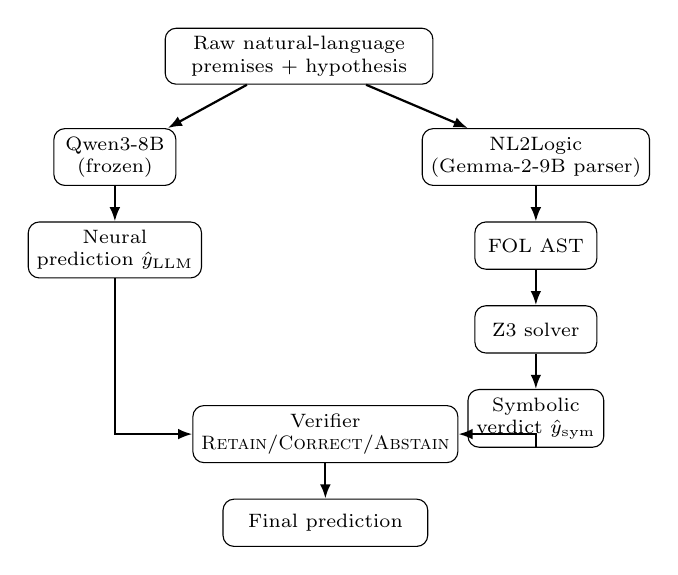
\begin{tikzpicture}[
  font=\scriptsize,
  box/.style={draw, rounded corners, align=center, minimum height=0.6cm, inner sep=3pt},
  arr/.style={-{Latex[length=1.8mm]}, thick}
]
\node[box, minimum width=3.4cm] (input) {Raw natural-language\\premises + hypothesis};

\node[box, below left=0.55cm and -0.15cm of input, minimum width=1.55cm] (qwen) {Qwen3-8B\\(frozen)};
\node[box, below right=0.55cm and -0.15cm of input, minimum width=1.55cm] (nl2logic) {NL2Logic\\(Gemma-2-9B parser)};

\node[box, below=0.45cm of qwen, minimum width=1.55cm] (ypred) {Neural\\prediction $\hat y_{\text{LLM}}$};
\node[box, below=0.45cm of nl2logic, minimum width=1.55cm] (ast) {FOL AST};
\node[box, below=0.45cm of ast, minimum width=1.55cm] (z3) {Z3 solver};
\node[box, below=0.45cm of z3, minimum width=1.55cm] (ysym) {Symbolic\\verdict $\hat y_{\text{sym}}$};

\node[box, below=0.9cm of $(ypred)!0.5!(ysym)$, minimum width=2.6cm] (verifier) {Verifier\\\textsc{Retain}/\textsc{Correct}/\textsc{Abstain}};
\node[box, below=0.45cm of verifier, minimum width=2.6cm] (final) {Final prediction};

\draw[arr] (input) -- (qwen);
\draw[arr] (input) -- (nl2logic);
\draw[arr] (qwen) -- (ypred);
\draw[arr] (nl2logic) -- (ast);
\draw[arr] (ast) -- (z3);
\draw[arr] (z3) -- (ysym);
\draw[arr] (ypred) |- (verifier);
\draw[arr] (ysym) |- (verifier);
\draw[arr] (verifier) -- (final);
\end{tikzpicture}
\caption{The dual-path NSCE architecture. The same raw text feeds a frozen neural branch (Qwen3-8B) and an independent neural-to-symbolic branch (NL2Logic with Gemma-2-9B, compiled to Z3); a deterministic verifier reconciles the two verdicts.}
\label{fig:architecture}
\end{figure}

\subsection{Neural Reasoning Branch}
A frozen Qwen3-8B~\cite{qwen3report} instance receives the raw premises and hypothesis through a fixed prompt template and produces one of \textsc{True}, \textsc{False}, or \textsc{Unknown} via constrained greedy decoding restricted to those three label tokens. The model is never fine-tuned, and no gold label or gold logical form is ever included in its prompt.

\subsection{Neural-to-Symbolic Bridge}
The same raw premises and hypothesis, sentence by sentence, are passed to the official NL2Logic framework~\cite{putra2026nl2logic}, using Gemma-2-9B-Instruct~\cite{gemma2report} as the semantic-parsing LLM inside NL2Logic's own recursive pipeline. For each sentence, NL2Logic's \texttt{ParserSelector} classifies it as atomic, quantified, or logical (connective-bearing), then recursively dispatches to a specialized sub-parser that extracts the outermost logical construct and re-feeds any remaining sub-sentence back into the parser, until each sentence is reduced to a first-order-logic abstract syntax tree (FOLAST). The upstream parser and AST-construction logic are NL2Logic's own design and are not modified or reimplemented. One harness-level addition was necessary to make its output executable: NL2Logic's generated entity and predicate names can be raw multi-word phrases (e.g., ``a bird''), which its own code generator splices verbatim into Python/Z3 source, producing a syntax error even on the framework's own published example. We added a deterministic identifier-sanitization step that rewrites such names into valid solver identifiers without altering the AST's logical structure; this is a harness-side, not an NL2Logic-side, change (Section~\ref{sec:models}).

\subsection{Symbolic Reasoning Layer}
Each sentence's FOLAST is compiled, via NL2Logic's deterministic two-pass generator, into declarations and expressions executable by the Z3 SMT solver~\cite{demoura2008z3}. We accumulate the per-sentence declarations and assertions for all premises of a given item into one shared Z3 solver context, and check entailment of the hypothesis $H$ against the conjoined premises $P$ using the standard three-way test:
\begin{equation}
\hat y_{\text{sym}} =
\begin{cases}
\text{TRUE}, & \text{if } P \wedge \neg H \text{ is UNSAT},\\
\text{FALSE}, & \text{if } P \wedge H \text{ is UNSAT},\\
\text{UNKNOWN}, & \text{otherwise.}
\end{cases}
\label{eq:verdict}
\end{equation}
If premise consistency itself is violated ($P$ is unsatisfiable) or any sentence fails to translate or compile, the item is flagged as a bridge failure rather than forced into one of the three labels.

\subsection{Verification and Feedback Layer}
A deterministic verifier (Algorithm~\ref{alg:verifier}) combines the neural prediction $\hat y_{\text{LLM}}$ and the symbolic verdict $\hat y_{\text{sym}}$. If the bridge failed to produce a verdict, the system \textsc{Abstain}s and reports the neural answer, explicitly unverified. If the two predictions agree, the system \textsc{Retain}s the neural answer. If they disagree, the system \textsc{Correct}s the neural answer with the symbolic verdict. This design deliberately does not simply replace the LLM with the solver: when the bridge fails, the frozen LLM's answer is still returned, rather than the pipeline failing outright.

\begin{algorithm}[t]
\caption{NSCE verification and feedback}
\label{alg:verifier}
\begin{algorithmic}[1]
\REQUIRE raw premises $p$, raw hypothesis $h$
\STATE $\hat y_{\text{LLM}} \gets \textsc{Qwen3-8B}(p, h)$ \COMMENT{Branch A, frozen}
\STATE $\text{ast} \gets \textsc{NL2Logic}(p, h)$ \COMMENT{Branch B, Gemma-2-9B parser}
\IF{translation or Z3 compilation of $\text{ast}$ fails}
    \STATE \textbf{return} $\hat y_{\text{LLM}}$, status $\gets$ \textsc{Abstain}
\ENDIF
\STATE $\hat y_{\text{sym}} \gets \textsc{SolveZ3}(\text{ast})$ \COMMENT{Eq.~\eqref{eq:verdict}}
\IF{$\hat y_{\text{LLM}} = \hat y_{\text{sym}}$}
    \STATE \textbf{return} $\hat y_{\text{LLM}}$, status $\gets$ \textsc{Retain}
\ELSE
    \STATE \textbf{return} $\hat y_{\text{sym}}$, status $\gets$ \textsc{Correct}
\ENDIF
\end{algorithmic}
\end{algorithm}

\section{Experimental Methodology}

\subsection{Research Questions}
\textbf{RQ1.} Can an independent symbolic verification branch improve a frozen LLM's predictions on raw natural-language logical reasoning, without modifying the LLM?\\
\textbf{RQ2.} How reliable is the neural-to-symbolic bridge under controlled, synthetic language versus more complex, natural language?\\
\textbf{RQ3.} When the neural and symbolic branches disagree, does the resulting correction help or harm accuracy?

\subsection{Datasets}
We use \textbf{ProofWriter}~\cite{tafjord2021proofwriter}, whose items consist of short, synthetic, closed-vocabulary facts and universally-quantified rules (e.g., ``If something is cold then it sees the lion.'') with minimal coreference, and \textbf{FOLIO}~\cite{han2024folio}, whose items are natural, crowd-sourced sentences with richer syntax, cross-sentence entity references, and more varied quantifier and connective structure. Both are used exactly as originally distributed as raw text; no gold FOL or gold labels are ever supplied to either branch. FOLIO evaluation uses items from the project's frozen 30-item FOLIO prototype sample; ProofWriter evaluation uses a non-frozen development pilot for gating and a separate frozen 20-item pilot sample for the headline comparison (Section~\ref{sec:results}), consistent with the project's own \texttt{proofwriter\_phase1\_samples=20} configuration.

\subsection{Models and Implementation Details}
\label{sec:models}
Branch A uses \textbf{Qwen3-8B}~\cite{qwen3report}, loaded once and reused unmodified across all items, with greedy (temperature-0) decoding constrained to the label set \{\textsc{True}, \textsc{False}, \textsc{Unknown}\}. Branch B uses the official \textbf{NL2Logic} implementation~\cite{putra2026nl2logic} with \textbf{Gemma-2-9B-Instruct}~\cite{gemma2report}, quantized to \texttt{Q4\_K\_M} (4-bit) and served through \textbf{Ollama}~\cite{ollama}, as its semantic-parsing model. Solving uses \textbf{Z3}~\cite{demoura2008z3} via the \texttt{z3-solver}~\cite{z3solver} Python bindings, with a 10-second per-check timeout. The identifier-sanitization step described in Section~\ref{sec:architecture} is the only harness-level addition to NL2Logic's own pipeline; it is applied uniformly regardless of dataset or outcome.

\subsection{Hardware}
All experiments ran on a single RTX~5050 Laptop GPU with approximately 8~GB of VRAM. The quantized Gemma-2-9B-Instruct model occupied approximately 6~GB and remained fully GPU-resident throughout; no CPU or shared-RAM offload was used or required.

\subsection{Metrics}
We report accuracy, macro-F1, per-class F1, AST validity rate, Z3-executability rate, verifier action counts (\textsc{Retain}/\textsc{Correct}/\textsc{Abstain}), helpful and harmful correction counts, and per-sentence translation latency (median, mean, and maximum, given the sensitivity of the mean to outliers observed in our runs).

\subsection{Leakage Prevention}
\label{sec:leakage}
Neither branch is ever given a gold label or gold logical form. Branch A's prompt contains only the raw facts, rules, and question/hypothesis. Branch B's translator receives only raw sentences; gold labels are used exclusively, after the fact, to score the already-produced predictions. The bridge's prompts, parser, and code generator are NL2Logic's own, unmodified aside from the identifier-sanitization step (Section~\ref{sec:architecture}), and none of it was tuned on any evaluation item.

\section{Results}
\label{sec:results}

\subsection{Bridge Evolution on FOLIO}

Table~\ref{tab:folio-evolution} summarizes every FOL-translation approach evaluated over the course of this study on FOLIO, prior to and including the NL2Logic bridge. Sample sizes differ across rows and are reported explicitly rather than merged into one column, because the 30-item and 5-item samples are not directly comparable in statistical power.

\begin{table}[t]
\caption{Bridge Evolution on FOLIO (sample sizes differ by row)}
\label{tab:folio-evolution}
\centering
\footnotesize
\setlength{\tabcolsep}{3pt}
\begin{tabular}{@{}lrrr@{}}
\toprule
Method ($n$) & AST valid & Z3-exec. & Verdict correct \\
\midrule
Gold-FOL oracle (30) & --- & --- & 29/30 (96.7\%) \\
Qwen3-8B V1, one-shot (30) & 9/30 & 8/30 & 4/30 (13.3\%) \\
Qwen3-8B V2, AST-guided (30) & 8/30 & 8/30 & 4/30 (13.3\%) \\
T5 bridge (5) & 3/5 & 3/5 & 0/5 (0\%) \\
NL2Logic+Gemma (5) & 29/29 sent. & 28/29 sent. & 1/5 (20\%) \\
\bottomrule
\end{tabular}
\vspace{2pt}
{\footnotesize\emph{Note:} NL2Logic's AST-valid/Z3-exec.\ counts are sentence-level; verdict correct is item-level throughout.}
\end{table}

The gold-FOL oracle row uses the officially provided logical forms rather than a model-produced translation; its 29/30 agreement with the frozen sample's labels indicates that our symbolic inference and label-mapping procedure (Eq.~\eqref{eq:verdict}) is largely consistent with the benchmark's own annotations when supplied with a correct formalization, not that Z3 itself was independently validated at scale. Two earlier Qwen3-8B translators -- a one-shot baseline (V1) and a decomposed, AST-inspired pipeline (V2) -- both plateau at 4/30 correct despite V2 sharply reducing malformed/schema errors (32$\to$2 sentences); quantifier-scope errors became V2's dominant failure category (32 occurrences), so V2 changed \emph{how} translation failed without improving \emph{how often} it was correct. A dedicated T5 bridge (\texttt{fvossel/t5-base-nl-to-fol}) was stopped under a predefined 5-item NO-GO gate at 0/5 semantically correct. NL2Logic with Gemma-2-9B achieves near-complete syntactic executability (28/29 sentences, 96.6\%) but only 1/5 correct final entailment verdicts -- a large jump in syntactic quality that did not carry through to semantic correctness (Section~\ref{sec:analysis}).

\subsection{FOLIO NL2Logic Gate}
On the 5-item FOLIO gate, drawn from the frozen 30-item prototype and covering binary-relation/multi-variable, universal-implication-with-negation, existential, conjunction/disjunction, and negation-with-binary-relation constructs, translation latency had a median of 12.1~s and a maximum of 30.2~s per sentence. No sentence timed out or crashed; the low verdict accuracy is a semantic, not an operational, failure (Section~\ref{sec:analysis}).

\subsection{Raw-Text ProofWriter Gate}
On a 5-item, non-frozen ProofWriter development-pilot gate, the same unmodified bridge (only the item loader differs, mapping ProofWriter's facts/rules/question format instead of FOLIO's premises/hypothesis format) achieved 5/5 valid ASTs, 5/5 Z3-executable theories, and 5/5 correct verdicts, at a median latency of 11.6~s/sentence. This gate passing decisively is what licensed proceeding to the frozen 20-item pilot below, under the same predefined go/no-go protocol that stopped the T5 bridge and (separately) the FOLIO branch of this study.

\subsection{Frozen 20-Item ProofWriter Pilot}
\label{sec:headline}
Table~\ref{tab:headline} reports the headline comparison on the frozen 20-item ProofWriter pilot. We term this a \emph{pilot}, not a benchmark evaluation, given $n=20$.

\begin{table}[t]
\caption{Frozen 20-item ProofWriter pilot: Qwen3-8B alone vs.\ full NSCE}
\label{tab:headline}
\centering
\begin{tabular}{@{}lrr@{}}
\toprule
Method & Accuracy & Macro-F1 \\
\midrule
Qwen3-8B only & 40.0\% (8/20) & 0.300 \\
\textbf{Full NSCE} & \textbf{70.0\% (14/20)} & \textbf{0.676} \\
\bottomrule
\end{tabular}
\end{table}

Full NSCE improves accuracy by an absolute \textbf{+30 percentage points} over Qwen3-8B alone. On this sample, the bridge translated and Z3-solved all 20 items successfully (0 bridge failures), and the standalone symbolic-branch accuracy is also 14/20 (70\%) -- a relationship we return to in Section~\ref{sec:analysis}, since it bears directly on how this gain should be attributed and on why the neural branch is retained at all rather than replaced by the bridge outright.

\begin{table}[t]
\caption{Verification actions on the frozen 20-item pilot}
\label{tab:verifier-actions}
\centering
\begin{tabular}{@{}lr@{}}
\toprule
Action & Count \\
\midrule
\textsc{Retain} & 14 \\
\textsc{Correct} & 6 \\
\textsc{Abstain} & 0 \\
\midrule
Helpful corrections & 6 \\
Harmful corrections & 0 \\
\bottomrule
\end{tabular}
\end{table}

Table~\ref{tab:verifier-actions} shows that of the 14 retained items, 8 were correct and 6 were cases where both branches agreed and were both wrong -- an upper bound the verifier cannot fix by construction, since it acts only on disagreement, not on shared error. All 6 disagreements were resolved by \textsc{Correct}ing toward the symbolic verdict, and every one of the 6 corrections was helpful; none were harmful. Treating this as paired data (Qwen wrong~$\rightarrow$~NSCE correct: 6; Qwen correct~$\rightarrow$~NSCE wrong: 0), an exact two-sided McNemar (sign) test on these 6 discordant pairs gives $p \approx 0.0313$. We report this descriptively, not as a well-powered confirmatory result: it is computed from only 6 discordant pairs out of a 20-item exploratory pilot, and the Wilson 95\% confidence intervals on the two underlying accuracy estimates are wide and overlapping (Qwen-only: $[21.9\%, 61.3\%]$; full NSCE: $[48.1\%, 85.5\%]$), which we discuss further as a direct consequence of $n=20$ in Section~\ref{sec:threats}.

\subsection{Latency}
On the frozen 20-item ProofWriter pilot, per-sentence translation latency had a median of 11.4~s and a mean of 22.9~s; the mean is pulled upward by a transient slowdown affecting four consecutive sentences during one stretch of the run, including one sentence with an outlier latency of approximately 2019~s. The precise cause of this slowdown was not established from the available logs. We report the median as the representative figure and discuss the outlier as an operational limitation in Section~\ref{sec:threats}, rather than treating the mean as representative.

\section{Analysis and Discussion}
\label{sec:analysis}

\textbf{Why ProofWriter works.} ProofWriter's sentences are short, use a small closed vocabulary, and express one relation per sentence with explicit universal quantification (``If something is X then it Y''). Each fact or rule maps almost directly onto NL2Logic's per-sentence unary/binary predicate scheme, so entities and predicates referenced in different sentences of the same item are far more likely to be named consistently, letting Z3 reason over a theory that actually reflects the source text.

\textbf{Why FOLIO does not, in our configuration.} FOLIO's sentences are longer, more syntactically varied, and more often depend on how an earlier sentence introduced or described an entity. In one worked FOLIO gate example (idx 180, gold label \textsc{False}), ``Susan flies \emph{to} LGA airport,'' ``The departure and arrival can not be the same airport,'' and ``John flies \emph{from} LGA airport'' each translate individually to syntactically valid, Z3-executable formulas, but the second sentence's constraint is captured as an unrelated unary predicate rather than as a relation linking the first and third sentences' airport arguments. The resulting theory is internally consistent but does not encode the cross-sentence constraint the premises actually assert, so Z3 correctly reports \textsc{Unknown} on a theory that was never given enough information to entail the true answer. This example, together with the aggregate gate numbers, suggests -- though $n=5$ cannot by itself prove -- that \textbf{executable logic does not imply semantically faithful logic}: syntactic executability rose from roughly 27\%~(8/30) for both Qwen3-8B translators to 96.6\%~(28/29 sentences) for NL2Logic, while verdict correctness on the FOLIO gate did not rise correspondingly (4/30~$\to$~1/5), consistent with NL2Logic's own noted limitation around co-reference and implicit cross-sentence links~\cite{putra2026nl2logic}.

\textbf{Why keep the neural branch, and how the gain should be attributed.} Because the bridge never failed on the ProofWriter pilot, every disagreement is by construction resolved toward the symbolic verdict, so the standalone symbolic-branch accuracy (14/20) exactly equals the full system's accuracy (14/20) -- a direct consequence of the bridge's reliability on this sample, not evidence that the \textsc{Retain}/\textsc{Correct}/\textsc{Abstain} policy itself is responsible for the +30-point gain. One might then ask why the frozen LLM is retained rather than using NL2Logic~+~Z3 alone. The neural branch serves purposes this pilot does not exercise: it is a general-purpose fallback on inputs outside the bridge's coverage (e.g., the FOLIO regime, or any item where translation/Z3 compilation fails and the system \textsc{Abstain}s); it supplies the disagreement signal needed to measure helpful versus harmful corrections, which a symbolic-only predictor cannot report on itself; and it is a prerequisite for future confidence-aware abstention (Section~\ref{sec:future}). On FOLIO, where the bridge is far less reliable in our configuration, we would not expect the same policy to produce a comparable gain, and we did not test the full NSCE loop there for this reason (Section~\ref{sec:threats}).

\section{Threats to Validity and Limitations}
\label{sec:threats}

\begin{itemize}
\item \textbf{Pilot sample size.} The headline comparison uses $n=20$ frozen items. The resulting Wilson confidence intervals on accuracy are wide and overlapping, and the exact McNemar test is computed on only 6 discordant pairs; none of this should be read as a well-powered benchmark result.
\item \textbf{ProofWriter is synthetic and closed-vocabulary.} The headline gain is demonstrated on language explicitly designed to be logically regular; we make no claim that it generalizes to less controlled text without further bridge work.
\item \textbf{FOLIO gate is small (5 items).} The 1/5 verdict-correct result, while consistent with the underlying translation failure mode we identify with a worked example, is itself too small a sample to bound a FOLIO-wide accuracy figure; we therefore report it as a documented limitation rather than as a benchmark score for NL2Logic on FOLIO, which the original NL2Logic publication evaluates at larger scale and reports considerably higher performance on~\cite{putra2026nl2logic}.
\item \textbf{Model- and quantization-specific results.} All symbolic-branch results use one specific quantized checkpoint (Gemma-2-9B-Instruct, Q4\_K\_M) under one serving stack (Ollama) on one 8~GB GPU. We did not test unquantized Gemma-2-9B, larger Gemma variants, or alternative parsing models within NL2Logic.
\item \textbf{Bridge dependence.} Because the bridge did not fail on the ProofWriter pilot, the full system's accuracy equals the symbolic branch's standalone accuracy on that sample (Section~\ref{sec:analysis}); the verifier's own distinct, attributable contribution here is its zero-harmful-correction property, not the headline accuracy delta.
\item \textbf{No confidence-aware correction yet.} The verifier applies the symbolic verdict on every disagreement, with no mechanism yet to weigh how trustworthy a given translation is before correcting (Section~\ref{sec:future}).
\item \textbf{Latency and operational robustness.} A single-worker queue with a purely advisory client-side timeout let one transient slowdown ($\sim$2019~s for one sentence, cause not established) inflate mean latency without aborting the run; a production system would need a hard, cancelling timeout and a multi-worker pool.
\item \textbf{No fine-tuning or larger-model comparison.} We do not compare against a fine-tuned Qwen3-8B or a larger frozen LLM (e.g., 70B-class), either of which might narrow or widen the observed gap.
\item \textbf{Possible reproduction differences from the original NL2Logic FOLIO setup.} Our item selection, prompt harness, and Z3 aggregation logic around NL2Logic's parser and generator (unmodified aside from Section~\ref{sec:architecture}'s identifier sanitization) may differ from the original paper's exact FOLIO protocol, partly explaining the gap between our 1/5 gate result and NL2Logic's own reported numbers; the two are not a like-for-like comparison.
\item \textbf{No claim of unrestricted natural-language success.} The positive result is demonstrated on a controlled synthetic dataset; we make no claim that the same gain holds on open-domain or unrestricted natural language.
\end{itemize}

\section{Future Work}
\label{sec:future}
Natural directions include: a larger held-out ProofWriter and FOLIO split once bridge reliability on the latter improves; reproducing NL2Logic's exact published FOLIO configuration to isolate our harness's contribution to the gap; explicit shared entity/relation normalization across sentences of an item (e.g., coreference resolution before parsing) to address the cross-sentence linking failure of Section~\ref{sec:analysis}; stronger or differently-quantized semantic-parsing models inside NL2Logic; calibrating the verifier's confidence rather than treating agreement/disagreement as binary; and bridge-confidence-aware abstention, so the system can decline to correct when the symbolic branch shows signs of a degenerate translation rather than only abstaining on outright failure.

\section{Conclusion}
On a small, frozen ProofWriter pilot ($n=20$), wiring an independent neural-to-symbolic-plus-solver verification branch around a frozen Qwen3-8B substantially improved its accuracy (40.0\%~$\to$~70.0\%) with zero observed harmful corrections, without any fine-tuning of the base model; because the bridge did not fail on this sample, this gain is best attributed to the reliability of the symbolic branch under a reliable bridge, rather than to the verifier policy alone. Our parallel, smaller FOLIO gate ($n=5$) shows that syntactic executability does not guarantee that reliability: NL2Logic with Gemma-2-9B produced valid, solver-executable logic on 96.6\% of FOLIO sentences yet only 1 of 5 correct downstream verdicts, consistent with cross-sentence semantic alignment -- rather than solver correctness or syntactic validity -- being a key observed bottleneck in this configuration. We report both results together, as an honest account of a verification architecture's limits is as important as its headline gain, and neither pilot is large enough to license claims beyond the specific configurations tested here.

\section*{Acknowledgment}
The authors thank the maintainers of NL2Logic, Z3, Qwen, Gemma, and Ollama for releasing the open models and tools this study depends on.

\bibliographystyle{IEEEtran}
\bibliography{references}

\end{document}
